\documentclass[12pt]{article} 
%\usepackage{times,helvet}
\usepackage{palatino}
%\usepackage[utf8]{inputenc} %useful to type directly diacritic characters
%\usepackage{ssss}
\usepackage{amsmath,amsbsy,amssymb}
\usepackage{sectsty,hangcaption}
\usepackage{deflist}
\usepackage{fancyhdr}
\usepackage{tabularx}
\usepackage{verbatim}
\usepackage{comment}
\usepackage{moreverb}
\usepackage{float,comment}
\usepackage{graphicx}
\usepackage{longtable}
%\usepackage{portland}
\usepackage{booktabs}

\usepackage[super,comma,sort]{natbib} 
\bibpunct[, ]{(}{)}{;}{a}{,}{,}

%must be last package
%\usepackage{hyperref}
\usepackage[debug=false, colorlinks=true, pdfstartview=FitV, linkcolor=blue, citecolor=blue, urlcolor=blue, pdfpagelabels=true]{hyperref}

\textwidth 6.5in
\textheight 9.5in
%\topmargin -.1in
\topmargin -.75in
\newlength{\boxwidth}
\setlength{\boxwidth}{5.8in}
\oddsidemargin -0in
\evensidemargin -0in
\headheight 0.25in

\lhead{{\sl PFLOTRAN: Governing Equations}}
\chead{\rm - \thepage\ -}
\rhead{\sl DRAFT: \today}
\cfoot{}

\newcommand\flotran{{\sl FloTran}}
\renewcommand{\baselinestretch}{1.0}
\def\EQ#1\EN{\begin{equation}#1\end{equation}}
\def\BA#1\EA{\begin{align}#1\end{align}}
\def\BS#1\ES{\begin{split}#1\end{split}}
%\newcommand{\EQ}{\begin{equation}}
%\newcommand{\EN}{\end{equation}}
\newcommand{\bcr}{\begin{center}}
\newcommand{\ecr}{\end{center}}
\newcommand{\eq}{\ =\ }
\newcommand{\degc}{$^\circ$C}
\renewcommand{\c}{{\rm CO_2}}
\newcommand{\im}{{\rm imb}}
\newcommand{\m}{{\rm mb}}
\newcommand{\ecm}{{\rm ecm}}
\newcommand{\eff}{{\rm eff}}
\newcommand{\eqr}{{\rm le}}
\newcommand{\equ}{{\rm eq}}
\newcommand{\kin}{{\rm kin}}
\newcommand{\rdx}{{\rm rdx}}
\newcommand{\ind}{{\rm id}}
\newcommand{\dep}{{\rm dp}}
\newcommand{\e}{{\rm{e}}}
\newcommand{\erf}{{\rm{erf}}}
\newcommand{\erfc}{{\rm{erfc}}}
\newcommand{\p}{{\partial}}
\newcommand{\A}{{\mathcal A}}
\newcommand{\B}{{\mathcal B}}
\newcommand{\C}{{\mathcal C}}
\newcommand{\D}{{\mathcal D}}
\newcommand{\E}{{\mathcal E}}
\newcommand{\F}{{\mathcal F}}
\newcommand{\G}{{\mathcal G}}
\newcommand{\I}{{\mathcal I}}
\newcommand{\J}{{\mathcal J}}
\newcommand{\M}{{\mathcal M}}
\newcommand{\cO}{{\mathcal O}}
\renewcommand{\P}{{{\mathcal P}}}
\newcommand{\Q}{{\mathcal Q}}
\newcommand{\R}{{{\mathcal R}}}
\renewcommand{\S}{{\mathcal S}}
\newcommand{\T}{{\mathcal T}}
\newcommand{\W}{{\mathcal W}}
\newcommand{\Y}{{\mathcal Y}}
\newcommand{\Z}{{\mathcal Z}}
\newcommand{\rev}{{\rm rev}}
\newcommand{\irr}{{\rm irr}}
\renewcommand{\a}{{\alpha}}
\newcommand{\abar}{{\bar \alpha}}
\renewcommand{\b}{{\beta}}
\renewcommand{\e}{{\epsilon}}
\newcommand{\s}{{\sigma}}
\renewcommand{\sc}{{g}}
\newcommand{\w}{{\rm H_2O}}
\newcommand{\air}{{\rm N_2}}
\newcommand{\pe}{{\rm Pe}}
\newcommand{\da}{{\rm Da}}
\renewcommand{\k}{{\dot R}^0}
\renewcommand{\L}{\widehat{\mathcal L}}
%\renewcommand{\bar}{\overline}
\newcommand{\dsty}{{\displaystyle}}
\newcommand{\diff}{{\mathcal D}}
\newcommand{\surf}{\equiv \!\!\!}
\newcommand{\bnabla}{\boldsymbol{\nabla}}
\newcommand{\ba}{\boldsymbol{a}}

\newcommand{\balpha}{\boldsymbol{\alpha}}
\newcommand{\bbeta}{\boldsymbol{\beta}}
\newcommand{\bgamma}{\boldsymbol{\gamma}}
\renewcommand{\d}{{\delta}}

\newcommand{\bA}{\boldsymbol{A}}
\newcommand{\bB}{\boldsymbol{B}}
\newcommand{\bb}{\boldsymbol{b}}
\newcommand{\bC}{\boldsymbol{C}}
\newcommand{\bc}{\boldsymbol{c}}
\newcommand{\bcolon}{\boldsymbol{:}}
\newcommand{\bdot}{\boldsymbol{\cdot}}
\newcommand{\bD}{\boldsymbol{D}}
\newcommand{\bE}{\boldsymbol{E}}
\newcommand{\bF}{\boldsymbol{F}}
\newcommand{\bG}{\boldsymbol{G}}
\newcommand{\bg}{\boldsymbol{g}}
\newcommand{\bi}{\boldsymbol{i}}
\newcommand{\bI}{\boldsymbol{I}}
\newcommand{\bJ}{\boldsymbol{J}}
\newcommand{\bK}{\boldsymbol{K}}
\newcommand{\bL}{\boldsymbol{L}}
\newcommand{\bM}{\boldsymbol{M}}
\newcommand{\bn}{\boldsymbol{n}}
\newcommand{\bdelta}{\boldsymbol{\delta}}
\newcommand{\bGamma}{\boldsymbol{\Gamma}}
\newcommand{\bomega}{\boldsymbol{\omega}}
\newcommand{\bOmega}{\boldsymbol{\Omega}}
\newcommand{\bPsi}{\boldsymbol{\Psi}}
\newcommand{\bO}{\boldsymbol{O}}
\newcommand{\bnu}{\boldsymbol{\nu}}
\newcommand{\bdS}{\boldsymbol{dS}}
\newcommand{\bP}{\boldsymbol{P}}
\newcommand{\bq}{\boldsymbol{q}}
\newcommand{\br}{\boldsymbol{r}}
\newcommand{\bR}{\boldsymbol{R}}
\newcommand{\bS}{\boldsymbol{S}}
\newcommand{\bU}{\boldsymbol{U}}
\newcommand{\bu}{\boldsymbol{u}}
\newcommand{\bv}{\boldsymbol{v}}
\newcommand{\bw}{\boldsymbol{w}}
\newcommand{\bx}{\boldsymbol{x}}
\newcommand{\by}{\boldsymbol{y}}
\newcommand{\bY}{\boldsymbol{Y}}
\newcommand{\bz}{\boldsymbol{z}}
\newcommand{\bzero}{\boldsymbol{0}}

\newcommand{\arrows}{~\rightleftharpoons~}
\newcommand{\arrowstab}{\!\!\!\rightleftharpoons\!\!\!}
\newcommand{\longline}{\noindent\rule[-0.1in]{\textwidth}{0.01in}}

\def\water{H$_2$O}
\def\calcium{Ca$^{2+}$}
\def\copper{Cu$^{2+}$}
\def\magnesium{Mg$^{2+}$}
\def\sodium{Na$^+$}
\def\potassium{K$^+$}
\def\uranium{UO$_2^{2+}$}
\def\hion{H$^+$}
\def\bicarbonate{HCO$_3^-$}
\def\cotwo{CO$_2$}
\def\chloride{Cl$^-$}
\def\fluoride{F$^-$}
\def\phosphoricacid{HPO$_4^{2-}$}
\def\nitrate{NO$_3^-$}
\def\sulfate{SO$_4^{2-}$}
\def\souotwooh{$>$SOUO$_2$OH}
\def\sohuotwocothree{$>$SOHUO$_2$CO$_3$}
\def\soh{$>$SOH}

%\renewcommand{\thepage}{\roman{page}}
%\renewcommand{\thepage}{\arabic{page}}
%\renewcommand{\theequation}{\arabic{section}.\arabic{subsection}-\arabic{equation}}
%\renewcommand{\theequation}{\arabic{section}-\arabic{equation}}
%\setcounter{page}{1}

\long\def\symbolfootnote[#1]#2{\begingroup%
\def\thefootnote{\fnsymbol{footnote}}\footnote[#1]{#2}\endgroup}

\setlength{\parindent}{0.3125in}
\setlength{\parskip}{2ex plus 0.2ex minus 0.2ex}

\setcounter{secnumdepth}{4}
\setcounter{tocdepth}{4}
\renewcommand{\contentsname}{CONTENTS}

\setlongtables

\pagestyle{fancy}

\thispagestyle{empty}

\author{P.C. Lichtner (LANL)}
\title{Requirements Document for H$_2$O--Supercritical CO$_2$ Two-Phase--Two-Component System}

\begin{document}

\maketitle

\tableofcontents

\section{Scope}

This report provides the governing equations, constitutive relations and numerical considerations for implementing the two-phase--two-component system H$_2$O--CO$_2$ into the SAMRAI parallel adaptive mesh refinement framework. Phases considered are liquid water (H$_2$O) and supercritical carbon dioxide (CO$_2$) designated as $\a = l,\, g$, respectively. Components consist of H$_2$O and CO$_2$ designated by the subscript $i=1,\,2$, respectively. The system considered may be either isothermal, in which case an energy balance equation is not necessary, or nonisothermal increasing the number of degrees of freedom by one.

Even this relatively simple system involves a complex system of nonlinear partial differential equations combined with complex equations of state for material properties and chemical solubility at the relevant temperatures and pressures.

\section{Governing Equations}

\subsection{Composition Variables}

There are several different approaches possible for solving the governing multiphase-multicomponent flow and transport equations depending on the choice of independent variables. The total number of independent variables is determined by the Gibbs phase rule. 
For a nonisothermal system derived from $N_P$ single fluid phases\symbolfootnote[2]{For a system with $N_P$ pure phases (e.g. $l$, $g$), there are $2^{N_P}\!-\!1$ possible phase combinations  (e.g. $l$, $g$, $lg$).} (e.g. $l$, $g$) and $N_C$ components (e.g. H$_2$O, CO$_2$), there are $N_C+1$ independent variables or degrees of freedom including temperature. 
Note that the number of degrees of freedom is independent of the number of possible phases in the system. To see this, the variables representing the system and the constraints imposed on the variables are listed in Table~\ref{tdof}.


\begin{table}[h]\centering
\caption{Variables and constraints in a multiphase-multicomponent system.}
\label{tdof}

\vspace{3mm}
%\renewcommand{\tabcolsep}{1cm}
\renewcommand{\arraystretch}{1.25}
\begin{tabular}{lccc}
\toprule
Variable & Number & Number & Constraint Condition\\
&Variables&Constraints&\\
\midrule
$T$ & 1 & 0 & ---\\
$P_\a$ & $N_P$ & $N_P\!-\!1$ & $P_{c,\a\b} = P_\b - P_\a$\\
$s_\a$ & $N_P$ & 1 & $\sum_\a s_\a=1$\\
$X_i^\a$ & $N_P N_C$ & $N_P$ & $\sum_i X_i^\a=1$\\
---&---& $N_C(N_P\!-\!1)$ & $\mu_i^\a = \mu_i^\b$\\
\midrule
Total: & $N_P(N_C+2)+1$ & $N_P (N_C + 2)-N_C$\\
\midrule
Net: & \multicolumn{2}{c}{$N_C+1$}\\
\bottomrule
\end{tabular}
\end{table}

For any particular control volume the quantity $n_i^\a$, equal to the number of moles of the $i$th component in phase $\a$, completely determines the chemical composition of the system. The total number of moles in phase $\a$, $n_\a$ is obtained by summing $n_i^\a$ over all components:
\EQ
N_\a \eq \sum_i n_i^\a.
\EN
The total number of moles in the system is then
\EQ
N \eq \sum_\a N_\a.
\EN
The mole fraction $X_i^\a$ of the $i$th species relative to phase $\a$ is thus defined as
\EQ\label{sumx}
X_i^\a \eq \frac{n_i^\a}{N_\a}, \ \ \ \ \ \ \ \sum_i X_i^\a =1.
\EN
Other composition variables may also be defined and are useful to what follows. The phase mole fraction $\zeta_\a$ is defined as
\EQ
\zeta_\a \eq \frac{N_\a}{N} \eq \dfrac{\displaystyle\sum\limits_i n_i^\a}{\displaystyle\sum_{i'\a'} n_{i'}^{\a'}}, \ \ \ \ \ \ \ \sum_\a \zeta_\a =1.
\EN
And the total component mole fraction $z_i$ is defined by
\EQ\label{sumzi}
Z_i \eq \frac{N_i}{N} \eq \dfrac{\displaystyle\sum_\a n_i^\a}{\displaystyle\sum_\a n_\a}, \ \ \ \ \ \ \ \sum_i Z_i=1.
\EN
These quantities are related by the expression
\EQ
Z_i \eq \frac{1}{N}\sum_\a n_i^\a \eq \sum_\a \frac{n_i^\a}{N_\a} \frac{N_\a}{N} \eq\sum_\a X_i^\a \zeta_\a.
\EN
It follows from the definition of $Z_i$ that
\EQ\label{zi}
Z_i \eq \dfrac{\displaystyle\sum_\a s_\a \rho_\a X_i^\a}{\displaystyle\sum_{\a} s_\a \rho_\a},
\EN
with molar density $\rho_\a$ and fluid volume fraction $s_\a$ for phase $\a$. The quantity $s_\a$ is defined as the ratio of fluid volume $V_\a$ of phase $\a$ to pore volume $V_p$
\EQ
s_\a \eq \frac{V_\a}{V_p},
\EN
and satisfies the relation
\EQ
\sum_\a s_\a \eq 1.
\EN
The pore volume $V_p$ is equal to the sum of all fluid phase volumes $V_\a$
\EQ
V_p \eq \sum_\a V_\a.
\EN
Eqn.\eqref{zi} then follows from the relations
\begin{subequations}
\BA
\frac{n_i^\a}{V} &\eq \frac{n_i^\a}{N_\a}\frac{N_\a}{V_\a}\frac{V_\a}{V_p}\frac{V_p}{V},\\
&\eq \varphi s_\a \rho_\a X_i^\a,
\EA
\end{subequations}
and
\begin{subequations}
\BA
\frac{N_\a}{V} &\eq \frac{N_\a}{V_\a}\frac{V_\a}{V_p}\frac{V_p}{V},\\
&\eq \varphi s_\a \rho_\a.
\EA
\end{subequations}
The formulation of the mass conservation equations in terms of $Z_i$ is used in the FLASH approach and avoids variable switching.

\subsection{Mass Conservation Equations}

The governing equations for mass conservation of each component $i$ can be written in the form
\EQ\label{massconv}
\sum_\a \left\{\frac{\p}{\p t} \big(\varphi s_\a \rho_\a X_i^\a\big) + \bnabla\cdot\bF_i^\a \right\} \eq Q_i,
\EN
with flux
\EQ
\bF_i^\a \eq \bq_\a \rho_\a X_i^\a -\varphi s_\a \rho_\a D_\a \bnabla X_i^\a,
\EN
consisting of contributions from advection and diffusion/dispersion.
In these equations $\varphi$ denotes the porosity, $s_\a$ the fluid volume fraction, $\rho_\a$ molar density, $D_\a$ diffusion/dispersion coefficient, and $X_i^\a$ mole fraction of the $i$th component in fluid phase $\a$. The quantity $Q_i$ denotes a source/sink term. The sum over $\a$ is over all fluid phases present in a particular control volume. 
The Darcy velocity $\bq_\a$ is given by the expression
\EQ
\bq_\a \eq -\frac{kk_\a}{\mu_\a} \bnabla \Big(P_\a - W_\a\rho_\a g z\Big),
\EN
for pressure $P_\a$ viscosity $\mu_\a$, formula weight $W_\a$, acceleration of gravity $g$, and elevation $z$.
The formula weight $W_\a$ for phase $\a$ consisting of a mixture of $N_C$ components is given by
\EQ
W_\a \eq \sum_i W_i X_i^\a,
\EN
where $W_i$ is the formula weight of the $i$th component. 

Introducing $Z_i$ into the mass conservation equations gives the alternative form
\EQ\label{mczi}
\frac{\p}{\p t} \Big(\varphi Z_i \sum_\a s_\a\rho_\a\Big) + \bnabla\cdot\sum_\a \bF_i^\a \eq Q_i.
\EN
In this equation the $N_C+1$ unknown variables are $(T, \, P,\, Z_1, \ldots,\, Z_{N_C})$, with one constraint among the variables $Z_i$. To solve the resulting system of equations it is necessary to express $s_\a$ and $X_i^\a$ as functions of $Z_i$. 

Summing Eqns.\eqref{massconv} or \eqref{mczi} over all components $i$ and making use of Eqn.\eqref{sumx} or Eqn.\eqref{sumzi} leads to the continuity equation
\EQ\label{masstot}
\sum_\a \left\{\frac{\p}{\p t} \big(\varphi s_\a \rho_\a \big) + \bnabla\cdot \big(\bq_\a \rho_\a \big)\right\} \eq Q,
\EN
with
\EQ
Q \eq \sum_i Q_i.
\EN
The equation for $i$ = H$_2$O in Eqn.\eqref{massconv} may be replaced with Eqn.\eqref{masstot}, for example, thereby eliminating the need to consider the diffusion term for H$_2$O.

\subsection{Energy Conservation}

The energy conservation equation can be written in the form
\EQ
\sum_\a\left\{\frac{\p}{\p t} \big(\varphi s_\a \rho_\a U_\a\big) + \bnabla\cdot\big(\bq_\a \rho_\a H_\a\big) \right\} + \frac{\p}{\p t} \big(\rho_r C_p T \big) - \bnabla\cdot\big(\kappa\bnabla T\big) \eq Q_e,
\EN
as the sum of contributions from each fluid phase and rock,
with internal energy $U_\a$ and enthalpy $H_\a$ of fluid phase $\a$, and rock heat capacity $C_p$ and thermal conductivity $\kappa$. The quantity $Q_e$ denotes the heat source/sink term. Internal energy and ethalpy are related through the thermodynamic expression
\EQ
H_\a \eq U_\a + \frac{P_\a}{\rho_\a}.
\EN

\section{Constitutive Relations}

\subsection{Material Properties}

Material fluid properties for density, viscosity, internal energy and enthalpy are needed for pure H$_2$O and supercritical CO$_2$, and in the case of nonisothermal systems internal energy and enthalpy. In addition, mixture properties for CO$_2$ dissolved in H$_2$O and H$_2$O dissolved in supercritical CO$_2$ are needed. 


Each phase $\a$ is a mixture of species H$_2$O and CO$_2$. 
%For H$_2$O, $W_{\rm H_2O} = 18.01534$ kg/mol, and for CO$_2$, $W_{\c} = 44.0098$ kg/kmol.


\subsubsection{Pure H$_2$O}

The density, viscosity, internal energy, and enthalpy of pure H$_2$O are taken from the steam tables [International Formulation Committee of the Sixth International Conference on Properties of Steam, (1967)] and is valid for the pressure and temperature range of $0 < P < 1000$ bars, and $0 < T < 800$\degc. In addition, the saturation curve of H$_2$O, $P_{\rm sat}(T)$ and its inverse relation $T_{\rm sat}(P_v)$, for vapor pressure $P_v$, are also provided.

\noindent
Critical temperature ($T_c$)	373.946\degc\\
Critical pressure ($P_c$)	220.640 bar\\
Critical density ($\rho_c$)	322.000000 kg/m$^3$\\
$W_{\rm H_2O} = 18.01534$ kg/mol

\subsubsection{Supercritical CO$_2$}

Material properties of supercritical CO$_2$ are obtained from an equation of state such as Span and Wagner (1996) for density, viscosity, internal energy, enthalpy, fugacity, and fugacity coefficient as functions of temperature and pressure.

\noindent
Critical temperature: ($T_c$) 30.9782\degc\\
Critical pressure: ($P_c$)	73.773 bar\\
Critical density: ($\rho_c$)	467.600 kg/m$^3$\\
$W_{\c} = 44.0098$ kg/kmol

\subsubsection{Mixture Properties}

\subsection{Capillary Pressure}

The pressure $P_\a$ of fluid phase $\a$ is related to the fluid pressure of phase $\b$ through the capillary pressure $P_{\a\b}^c$
\EQ
P_{\a\b}^c \eq P_\b - P_\a,
\EN
where $P_\b$ is assumed to be the non-wetting phase, in this case supercritical CO$_2$, and $P_\a$ refers to the wetting phase in this case brine. Capillary pressure is related to saturation $s_\a$ using, for example, van Genuchten or Brooks-Cory correlations.

\subsection{Supercritical CO$_2$--H$_2$O Equilibrium Relations}
\label{sec:eqrel}

For an aqueous fluid in equilibrium with supercritical CO$_2$ it is necessary to use an equation of state for CO$_2$ to obtain the solubility of CO$_2$ in solution. The presentation follows Duan and Sun (2003). 

Equilibrium of supercritical CO$_2$ with an aqueous solution is described by the reactions
\begin{subequations}
\EQ\label{co2}
{\rm CO}_2^l \arrows {\rm CO}_2^g,
\EN
and
\EQ\label{h2o}
{\rm H_2O}^l \arrows {\rm H_2O}^g.
\EN
\end{subequations}
The mass action equation corresponding to reaction \eqref{co2} is given by
\EQ\label{massactco2}
K_\c^{\rm eq} \eq \frac{f_\c^{}}{a_\c^{\rm eq}} 
\eq \frac{\phi_\c^{} P_\c^g}{a_\c^{\rm eq}} 
\eq \frac{\phi_\c^{} X_\c^g P_g^{}}{a_\c^{\rm eq}},
\EN
with equilibrium constant $K_\c^{\rm eq}$.
The activity of $\c$ in the aqueous solution is related to its molality $m_\c^{\rm eq}$ by
\EQ
a_\c^{\rm eq} \eq \gamma_\c^{\rm eq} m_\c^{\rm eq},
\EN
where $\gamma_\c$ denotes the activity coefficient.
The fugacity is given by
\EQ
f_\c^{} \eq \phi_\c^{} P_\c^{g} \eq \phi_\c^{} X_\c^g P_g^{},
\EN
with fugacity coefficient $\phi_\c$, where the mole fraction of $\c$ in the supercritical (gas) phase, $X_\c^g$, is assumed to be given by
\EQ\label{xco2g}
X_\c^g \eq \frac{P_\c^g}{P_g} \eq \frac{P_g-P_\w^{\rm sat}(T)}{P_g} \eq 1-\frac{P_\w^{\rm sat}(T)}{P_g},
\EN
with total gas pressure $P_g$ equal to
\EQ\label{totalp}
P_g \eq P_\c^g + P_\w^{\rm sat}(T),
\EN
and where $P_\w^{\rm sat}(T)$ denotes the saturation pressure of pure water. 
The equilibrium concentration of CO$_2$ in the aqueous solution in terms of molality units is thus given by
\EQ
m_\c^{\rm eq} \eq \frac{\phi_\c^{} X_\c^g}{\gamma_\c^{}K_\c^{\rm eq}}  P_g^{}.
\EN
Molality is related to mole fraction $X_\c^{l,{\rm eq}}$ by the equation
\begin{subequations}
\EQ\label{xco2l}
X_\c^{l,{\rm eq}} \eq\frac{W_\w m_\c^{\rm eq}}{1 + W_\w m_\c^{\rm eq}},
\EN
and conversely mole fraction is related to molality by the inverse relation
\EQ
m_\c^{\rm eq} \eq \frac{X_\c^{l,{\rm eq}}}{W_\w(1-X_\c^{l,{\rm eq}})},
\EN
\end{subequations}
where $W_\w$ denotes the formula weight of water. 

\subsection{Phase Change Criteria}

In the FLASH approach the primary variables are $P$, $T$ and the total mole fraction $Z_i$ of the $i$th component summed over all phases.
This gives $2+N_C-1 = N_C+1$ independent variables as required. The variable $Z_i$ is a persistent degree of freedom throughout the simulation. From the knowledge of $Z_i$ it is possible to obtain the stable phase assemblage, the volume fraction $s_\a$ of each phase present in the system, and its composition in terms of $X_i^\a$. 

For a two-phase ($\a=l$, $\sc$) system where, for example, $l$ designates the liquid phase $\w$ and $\sc$ designates supercritical $\c$, $Z_i$ can be expressed as
\EQ
Z_i \eq \frac{\rho_l^{} s_l^{} X_i^l + \rho_{\sc}^{} s_{\sc}^{} X_i^{\sc}}{\rho_l^{} s_l^{} + \rho_{\sc}^{} s_{\sc}^{}},
\EN
for molar fluid densities $\rho_l$, $\rho_{\sc}$ and phase saturation $s_l$, $s_{\sc} = 1\!-\!s_l$.
Solving for $s_g$ gives
\EQ\label{sg}
s_g \eq \frac{\rho_l(Z_i^{}-X_i^l)}{\rho_l(Z_i^{} - X_i^l) - \rho_g (Z_i^{} -X_i^g)}, \ \ \ \ \ (i= {\rm H_2O,\, CO_2}).
\EN

To determine the mole fractions $X_i^\a$ from $Z_i$ it is necessary to consider the equilibrium constraints between phases expressed as equality their chemical potentials in the two phases.

Depending on the value of $Z_\c$ different phases are present in the system.
\begin{description}
\item[Single Liquid Phase:] For $Z_\c \!<\! X_\c^{l,{\rm eq}}$, a single aqueous ($\w$) phase is the stable phase assemblage.
The aqueous $\c$ concentration is equal to
\begin{subequations}\label{fla-sec-c1}
\BA\label{liq}
X_i^l = Z_i^{},
\EA
and phase saturations are given by
\BA
s_l = 1, \ s_{\sc} =0,
\EA
\end{subequations}
consistent with Eqn.\eqref{sg}.

\item[Single Gas Phase:] For $Z_\c\!>\! X_\c^{g,\rm eq} \!=\!1\!-\!P_\w^{\rm sat}(T)/P_g$, a single supercritical $\c$ phase is the stable phase assemblage.
The supercritical $\c$ concentration is equal to
\begin{subequations}\label{fla-sec-c2}
\BA\label{gas}
X_i^{\sc} = Z_i^{},
\EA
and phase saturations are given by
\BA
 s_l = 0, \ s_{\sc} =1,
\EA
\end{subequations}
consistent with Eqn.\eqref{sg}.

\item[Two-Phase:] For $Z_\c \!>\! X_\c^{l,{\rm eq}}$ and $Z_\c\!<\! X_\c^{g,{\rm eq}}\!=\!1\!-\!P_\w^{\rm sat}/P_g$, the two phases supercritical $\c$ and a liquid phase coexist.
From Section \ref{sec:eqrel} the equilibrium mole fractions of CO$_2$ in the liquid and gas phases are given by Eqns.\eqref{xco2l} and \eqref{xco2g}, respectively.
Note that the equilibrium composition only depends on temperature and pressure and is independent of $Z_\c$, and thus forms an invariant composition. The gas saturation is determined from Eqn.\eqref{sg}
\EQ\label{2ph}
s_{\sc} \eq \frac{\rho_{l} (Z_{\c}^{} - X_{\c}^{l,\rm eq})}
{\rho_l (Z_{\c}^{} - X_{\c}^{l,\rm eq}) - \rho_{\sc} (Z_{\c}^{} - X_{\c}^{\sc})},
\EN
with $s_l\!=\!1\!-\!s_{\sc}$.
The density of either the aqueous or supercritical $\c$ phase is obtained from an equation of state, as a function of $P$, $T$ and $X_i^{l,\,g}$, based on the mixture density for the phase.
\end{description}

\section{Numerical Implementation}

\subsection{Independent Variables}

In the following the so-called Flash method is used in which a persistent set of independent variables exist regardless of the which phases are present in the system within any particular control volume and time $t$. This approach is advantageous for use with multilevel solvers to avoid changes in the independent variables on different levels within a patch as could occur in the variable switching approach.
Significant simplifications are possible for a two-phase--two-component system such as characterizes the liquid plus supercritical CO$_2$ system considered here. For this system $N_P=2$ $(l,\,g)$, and $N_C=2$ $(\rm H_2O,\, CO_2)$. Three distinct states exist in the system corresponding to single liquid, single gas and two-phase liquid-gas states. The three independent variables are taken as $P$, $T$, and $Z_\c$.

\subsection{Finite Volume Discretization}

\subsubsection{Residual Function}

Using a finite volume discretization approach, the governing flow and transport equations are discretized according to a sum of accumulation, flux and source/sink terms providing the residual function $R_{in}$ for the $i$th component at the $n$th control volume and $k+1$st time step $\Delta t_{k+1}$ given by
\BA
R_{in}^{k+1} \eq & \left[\big(\varphi  Z_i\sum_\a s_\a \rho_\a\big)_n^{k+1}-(\varphi Z_i\sum_\a s_\a\rho_\a)_n^k \right] \frac{V_n}{\Delta t_{k+1}} 
+ \sum_{\a n'} (F_i^\a )_{nn'}^{k+1} A_{nn'}
- Q_{in}^{k+1} V_n,
\EA
formulated in terms of the primary variables $T,\, P,\, Z_i$ for use with the flash approach.
In this equation the sum over $n'$ is over all control volumes which are connected to the $n$th control volume with volume $V_n$ and interfacial area $A_{nn'}$. The discritzed form of the flux $(F_{i^\a})_{nn'}^{k+1}$ is given by
\EQ
(F_i^\a)_{nn'}^{k+1} \eq (q_{\a}\rho_{\a}X_{i}^{\a})_{nn'}^{k+1} -(\varphi s_{\a} \rho_\a D_\a)_{nn'}^{k+1} \frac{X_{i n'}^{\a, k+1}-X_{i n}^{\a,k+1}}{d_{n'}+d_n},
\EN
consisting of contributions from advection and diffusion, where the distances $d_n$, $d_{n'}$ refer to the perpendicular distance from the control volume center to the interface. Special consideration is necessary for quantities evaluated at the interface $n\!-\!n'$ denoted by $(~)_{nn'}$.
In evaluating the residual function the quantities $s_\a$ and $X_i^\a$ are expressed as functions of $Z_i$.

By summing over all components and making use of the constraint condition Eqn.\eqref{sumzi} it is possible to eliminate one residual component equation and replace it with the pressure equation
\BA
R_{n}^{k+1} \eq &\sum_\a \Big[\big(\varphi s_\a \rho_\a)_n^{k+1} -(\varphi s_\a \rho_\a)_n^k \Big] \frac{V_n}{\Delta t_{k+1}} + \sum_{\a n'} (F_\a )_{nn'}^{k+1} A_{nn'}- Q_{n}^{k+1} V_n,
\EA
with
\EQ
(F_\a)_{nn'}^{k+1} \eq \sum_i (F_i^\a)_{nn'}^{k+1} \eq (q_{\a}\rho_{\a})_{nn'}^{k+1},
\EN
where
\EQ
R_n \eq \sum_i R_{in},
\EN
and
\EQ
Q_n \eq \sum_i Q_{in}.
\EN

\subsubsection{Interface Properties}

Shown in Table~\ref{tinterface} is the interface averaging assumption made for each quantity listed.

\begin{table}[h]\centering
\caption{Interface Property}\label{tinterface}

\vspace{3mm}

\renewcommand{\arraystretch}{2}
\begin{tabular}{lccc}
\toprule
Property & Symbol(s) & Average & Expression\\
\midrule
Permeability & $k$ & Harmonic & $\dfrac{k_1 k_2(d_1+d_2)}{d_1 k_2 + d_2 k_1}$\\
\midrule
Mole Fraction & $Z_i$ & Upwinding & $Z_{i,nn'} = Z_{in}, \ q_{nn'}>0$\\
&&&$Z_{i,nn'} = Z_{in'}, \ q_{nn'}<0$ \\
\midrule
Density & $\rho_\a$ & Arithmetic & $\dfrac{d_2\rho_2 + d_1\rho_1}{d_1+d_2}$\\
\midrule
Diffusion & $s_\a\tau_\a D_\a$ & Harmonic & $\dfrac{(s_\a\tau_\a D_\a)_1(s_\a\tau_\a D_\a)_2 (d_1+d_2)}{d_2(s_\a\tau_\a D_\a)_1 + d_1(s_\a\tau_\a D_\a)_2}$\\
\bottomrule
\end{tabular}
\end{table}

\subsubsection{Jacobian Matrix}

The Jacobian matrix for an isothermal system has the form
\EQ
\renewcommand{\arraystretch}{2.0} 
\bJ \eq 
\begin{bmatrix}
\dfrac{\p R_P}{\p P} & \dfrac{\p R_P}{\p Z} \\
\dfrac{\p R_Z}{\p P} & \dfrac{\p R_Z}{\p Z}
\end{bmatrix}.
\EN
For a nonisothermal system there is an addition equation for the temperature
\EQ
\renewcommand{\arraystretch}{2.0} 
\bJ \eq 
\begin{bmatrix}
\dfrac{\p R_p}{\p P} & \dfrac{\p R_p}{\p T} & \dfrac{\p R_p}{\p Z} \\
\dfrac{\p R_T}{\p P} & \dfrac{\p R_T}{\p T} & \dfrac{\p R_T}{\p Z} \\
\dfrac{\p R_Z}{\p P} & \dfrac{\p R_Z}{\p T} & \dfrac{\p R_Z}{\p Z}
\end{bmatrix}.
\EN


\section{Example Problem}

An example problem using PFLOTRAN is presented to provide a benchmark problem for comparison with SAMRAI. In this problem supercritical CO$_2$ is injected at a rate of 1 kg/s for 10 years at the center of a domain of size 500 m $\!\times\!$ 500 m $\!\times\!$ 100 m in a grid cell measuring 10 m $\!\times\!$ 10 m $\!\times\!$ 2 m. A coarse grid is used with size 25 $\times$ 25 $\times$ 50. The ambient temperature is taken as 50\degc\ with a pressure of 200 bars.

Results are shown in Figures~\ref{f10y} and \ref{f250y} for times of 10 and 250 years, respectively, for saturation (left) and dissolved CO$_2$ (right). Fingering of dissolved CO$_2$ occurs in the H$_2$O phase as evident in Figure~\ref{f250y}.

Shown in Figure~\ref{fmass} is the total moles of CO$_2$ in the H$_2$O (blue curve) and supercritical CO$_2$ (red curve) phases. The peak in CO$_2$ in the supercritical CO$_2$ phase occurs at 10 years when injection is halted. With increasing time the CO$_2$ in the H$_2O$ increases with time and the supercritical CO$_2$ phase dissipates.

\begin{figure}[h]
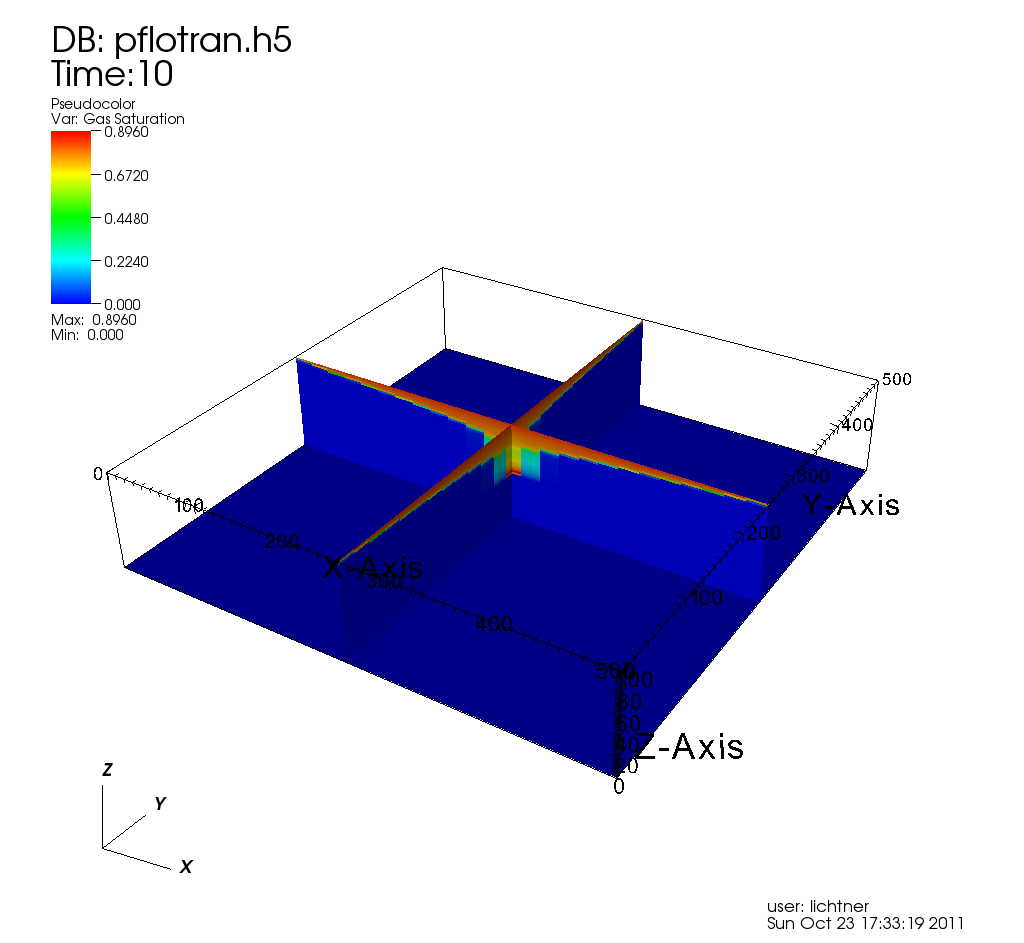
\includegraphics[scale=0.25]{./figs/sg-10y.png}
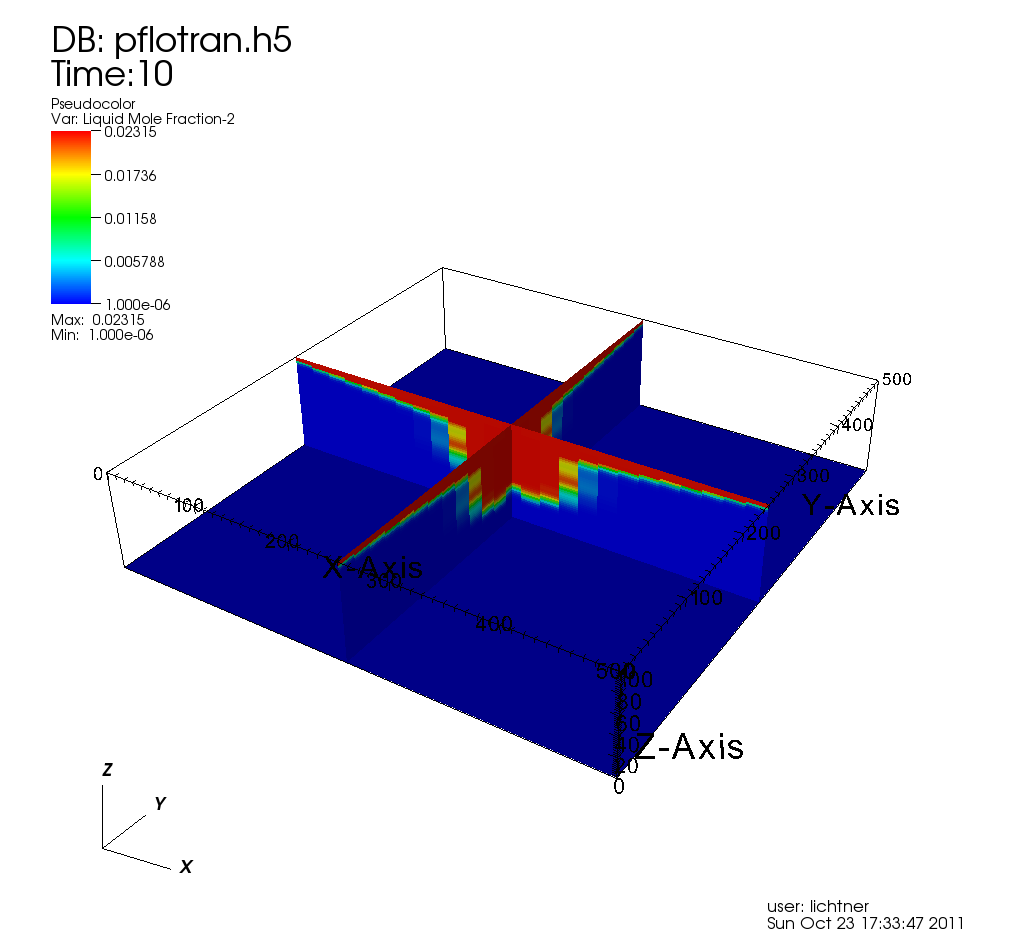
\includegraphics[scale=0.25]{./figs/xlco2-10y.png}
\caption{Saturation of supercritical CO$_2$ (left) and mole fraction of dissolved CO$_2$ (right) at an elapsed time of 10 years when injection is halted.}\label{f10y}
\end{figure}

\begin{figure}
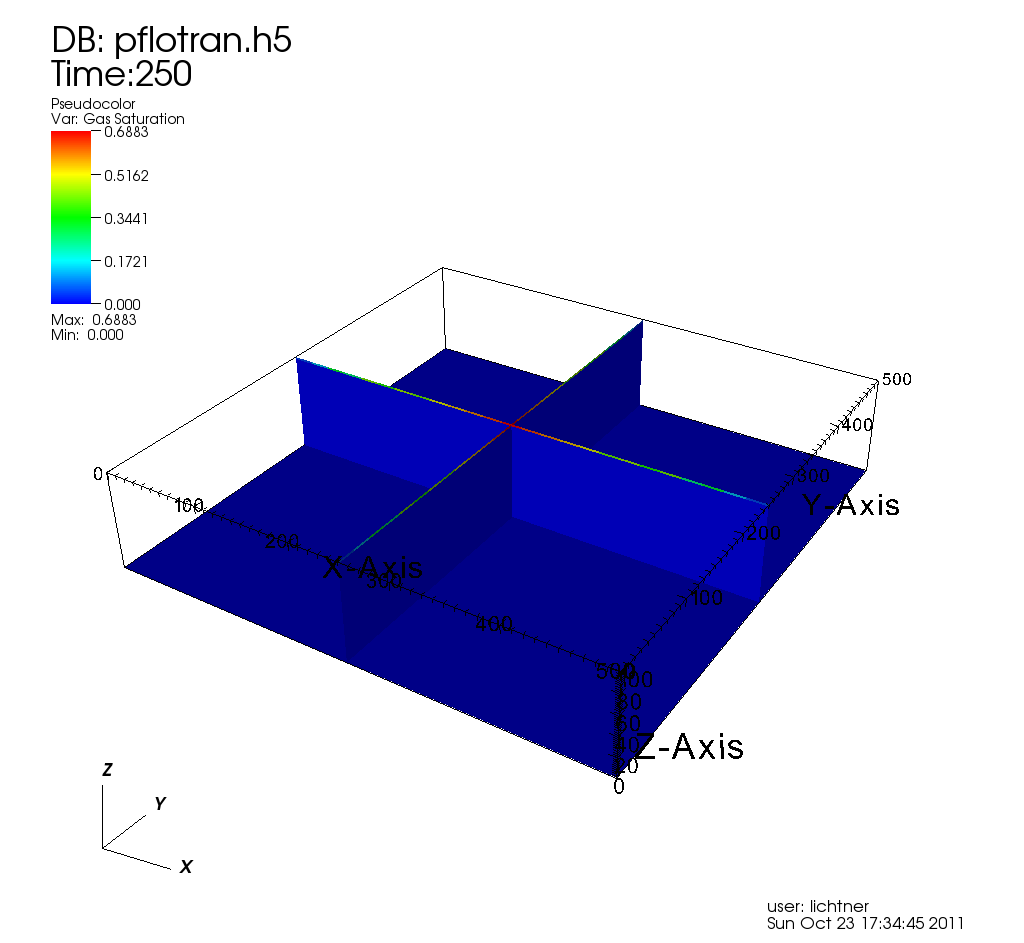
\includegraphics[scale=0.25]{./figs/sg-250y.png}
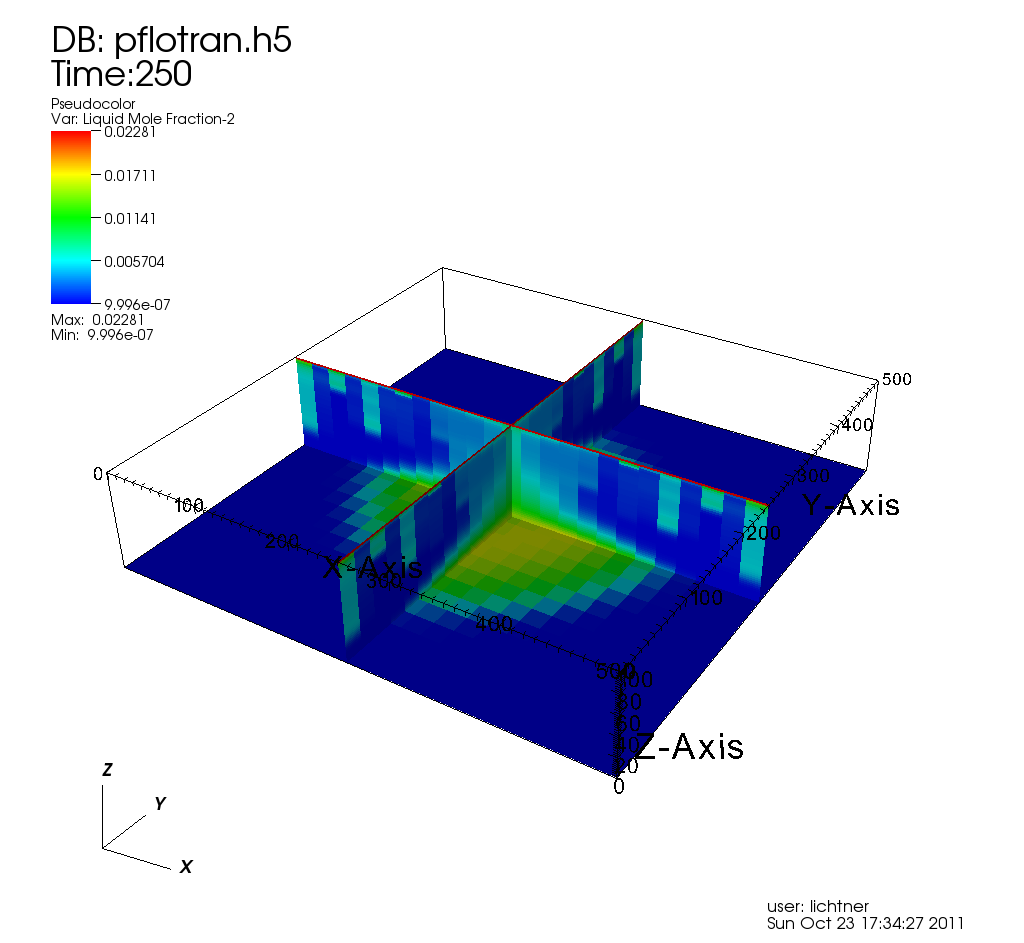
\includegraphics[scale=0.25]{./figs/xlco2-250y.png}
\caption{Saturation of supercritical CO$_2$ (left) and mole fraction of dissolved CO$_2$ (right) at an elapsed time of 250 years.}\label{f250y}
\end{figure}

\begin{figure}\centering
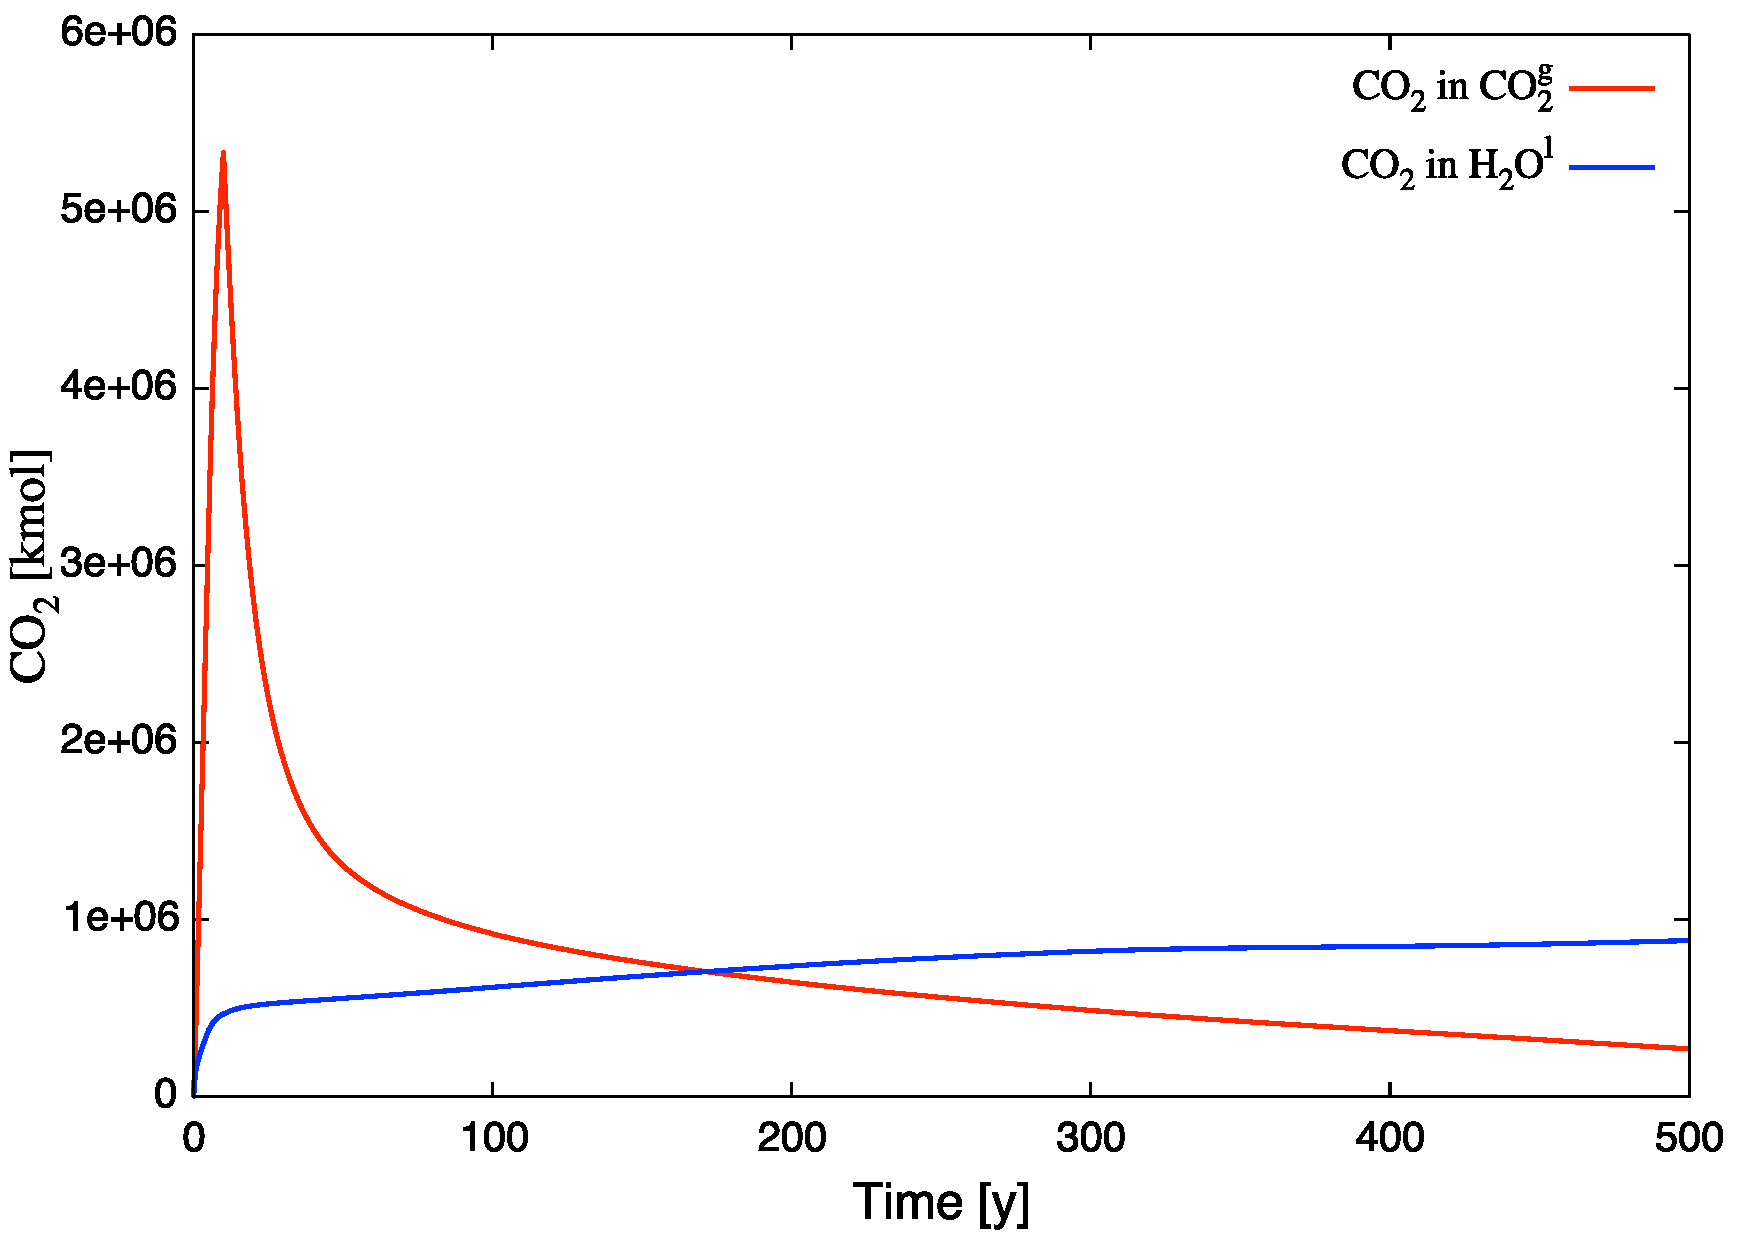
\includegraphics[scale=0.45]{./figs/mass}
\caption{Moles of CO$_2$ as a function of time in H$_2$ and supercritical CO$_2$ phases.}\label{fmass}
\end{figure}

\newpage
\section{References}

Span, R., Wagner, W. (1996) A New Equation of State for Carbon Dioxide Covering the Fluid Region from the Triple-Point Temperature to 1100 K at Pressures up to 800 MPa, J. Phys. Chem. Ref. Data, 25, 6, 1509--1596.

Revised Release on the IAPS Formulation 1985 for the Thermal Conductivity of Ordinary Water Substance, International Association for the Properties of Water and Steam, London, 1998, 23. 

Thermal conductivity and viscosity

Kestin, J.; Sengers, J.V.; Kamgar-Parsi, B.; Levelt Sengers, J.M.H., Thermophysical Properties of Fluid H2O, J. Phys. Chem. Ref. Data, 1984, 13, 1, 175-183.

Viscosity

IAPWS, Revised Release on the IAPS Formulation 1985 for the Viscosity of Ordinary Water Substance, International Association for the Properties of Water and Steam, Erlangen, Germany, 1997, 15.

\bibliographystyle{plainnat}
\bibliography{./reference-new}


\end{document}

Activity coefficients and standard state potentials are related by
\BA
\mu_i &\eq \mu_i^m + RT \ln \gamma_i m_i,\\
&\eq \mu_i^x + RT \ln \lambda_i x_i,
\EA
with [see Denbigh (1981), p. 278, Eqns.(9$\cdot$19) and (9$\cdot$20)]
\EQ
\gamma_i \eq x_w \lambda_i,
\EN
and
\EQ
\mu_i^m \eq \mu_i^x + RT \ln W_w.
\EN

The concentration of $\c$ in the gas phase, $C_\c^g$, is obtained as
\BA
C_\c^g &\eq \frac{n_i^g}{V_g} \eq \frac{n_i^g}{N_g}\frac{N_g}{V_g} \eq \rho_\c^{} X_\c^g,\\
&\eq \rho_\c \frac{f_\c}{\phi_\c P_g},\\
&\eq \rho_\c K_\c^{\rm eq} \frac{a_\c}{\phi_\c P_g}.
\EA


In the general case molality and mole fraction of solute species $i$ are related by the expressions
\EQ
m_i \eq \frac{x_i}{W_w x_w} \eq \frac{x_i}{W_w(1-\sum_{l\ne w} x_l)},
\EN
and the inverse relation
\EQ
x_i \eq \frac{W_w m_i}{1+W_w \sum_{l\ne w} m_l},
\EN
where $x_w$ and $W_w$ denote the mole fraction and formula weight of the solvent, in this case $\w$, respectively, with
\EQ
x_w \eq \frac{1}{1+W_w \sum_{l\ne w} m_l}.
\EN

implies equality of the chemical potentials
\EQ
\mu_\c^l \eq \mu_\c^g,
\EN
where
\EQ
\mu_\c^l \eq \mu_\c^{\ominus l} + RT\ln a_\c^{},
\EN
and
\EQ
\mu_\c^g \eq \mu_\c^{\ominus g} + RT\ln f_\c^{},
\EN
with standard state chemical potentials $\mu_\c^{\ominus l}$ and $\mu_\c^{\ominus g}$. The activity of $\c$ in an aqueous solution is related to its molality $m_\c$ by
\EQ
a_\c^{} \eq \gamma_\c^{} m_\c^{},
\EN
where $\gamma_\c$ denotes the activity coefficient for aqueous $\c$.
The fugacity is given by
\EQ
f_\c^{} \eq \phi_\c^{} P_\c^{} \eq \phi_\c^{} X_\c^g P_g^{},
\EN
with fugacity coefficient $\phi_\c$ where the mole fraction of $\c$ in the supercritical (gas) phase, $X_\c^g$, is assumed to be given by
\EQ
X_\c^g \eq \frac{P_\c^g}{P_g} \eq \frac{P_g-P_\w^{\rm sat}(T)}{P_g} \eq 1-\frac{P_\w^{\rm sat}(T)}{P_g},
\EN
with total gas pressure $P_g$ equal to
\EQ\label{totalp}
P_g \eq P_\c^g + P_\w^{\rm sat}(T),
\EN
and where $P_\w^{\rm sat}(T)$ denotes the saturation pressure of pure water. 

Introducing the equilibrium constant $K_\c^{\rm eq}$ defined as
\EQ
\ln K_\c^{\rm eq} \eq -\frac{1}{RT}\big(\mu_{\rm CO_2}^{g\ominus} - \mu_{\rm CO_2}^{l\ominus}\big),
\EN
yields the mass action equation
\EQ\label{massactco2}
K_\c^{\rm eq} \eq \frac{f_\c^{}}{a_\c^{}} \eq \frac{\phi_\c^{} P_\c^g}{a_\c} \eq \frac{\phi_\c^{} X_\c^g P_g^{}}{a_\c^{}}.
\EN
The equilibrium CO$_2$ molality is thus given by
\EQ
m_\c^{} \eq \frac{\phi_\c^{} X_\c^g}{\gamma_\c^{}K_\c^{\rm eq}}  P_g^{}.
\EN
%Of the three quantities: $P_g$, $P_\c^g$, and $T$, two may be specified and the other computed from Eqn.\eqref{totalp}.
Solving Eqn.\eqref{massactco2} for the $\c$ partial pressure gives
\BA
P_\c^g &\eq \frac{K_\c^{\rm eq}}{\phi_\c} a_\c,\\
&\eq \widetilde K_\c^{\rm eq} a_\c,
\EA
where the effective equilibrium constant $\widetilde K_\c$ is defined as
\EQ
\widetilde K_\c^{\rm eq} \eq \frac{K_\c^{\rm eq}}{\phi_\c}.
\EN

For a two-component system $\w$, $\c$, molality is related to the mole fraction by the equation
\begin{subequations}
\EQ
x_\c^l \eq\frac{W_\w m_\c}{1 + W_\w m_\c},
\EN
and conversely mole fraction is related to molality by the inverse relation
\EQ
m_\c \eq \frac{x_\c^l}{W_\w(1-x_\c^l)},
\EN
\end{subequations}
where $W_\w$ denotes the formula weight of water. 

\BA
R_{in}^{k+1} \eq &\sum_\a \left\{\frac{\big(\varphi s_\a \rho_\a X_i^\a\big)_n^{k+1}-(\varphi s_\a \rho_\a X_i^\a)_n^k}{\Delta t_{k+1}} \right\} V_n \nonumber\\
& + \sum_{\a n'} (F_i^\a )_{nn'}^{k+1} A_{nn'} \nonumber\\
&- Q_{in}^{k+1} V_n,
\EA


\subsubsection{Two-Component System}

\begin{comment}
One important assumption in the implementation in PFLOTRAN is that the activity coefficients in the aqueous phase and the fugacity coefficient in the supercritical phase are not functions of the $\c$ concentration. 
%I.e. non-ideality is weak in the aqueous and gas mixtures. 
This assumption is consistent with the solubility equations for $\c$ [\cite {garcia01}, \cite{duan2003}, \cite{duan2008}] adapted in PLOTRAN. With this assumption, the phase distribution parameters $K_i(P,\,T)$ are not functions of the mole fractions $z_i, x_i$ and $y_i$, which greatly simplifies the flash calculation. 
\end{comment}

Currently the FLASH2 mode in PFLOTRAN can only handle systems with two components and two phases, enabling the flash calculation to be carried out in a simplified manner. 
For a two-component system the FLASH equations may be solved analytically. 
In this case, with the notation $x_i = X_i^l$ and $y_i = X_i^g$, there are four constraint conditions in four unknowns ($x_1,\,x_2,\,y_1,\,y_2$):
\begin{subequations}
\EQ
y_i=K_ix_i,
\EN
\EQ
x_1+x_2\eq 1,
\EN
and
\EQ
y_1+y_2 \eq K_1 x_1 + K_2 x_2 \eq 1,
\EN
\end{subequations}
These equations have the solution
\begin{subequations}
\EQ
x_1 = \frac{1-K_2}{K_1-K_2}, \ \ \ x_2=1-x_1 \eq \frac{K_1-1}{K_1-K_2},
\EN
and
\EQ
y_1 = \frac{K_1(1-K_2)}{K_1-K_2}, \ \ \ y_2 \eq \frac{K_2(K_1-1)}{K_1-K_2}.
\EN
\end{subequations}
The gas phase mole fraction $\zeta_g$ can then be obtained from the equation
\EQ
Z_i \eq (1-\zeta_g) x_i + \zeta_g K_i x_i,
\EN
to give
\begin{subequations}
\BA
\zeta_g &\eq \frac{Z_i - x_i}{(K_i-1)x_i}, \ \ \ \ \ (i=1,\,2),\\
&\eq \frac{Z_1(K_1-K_2)-(1-K_2)}{(K_1-1)(1-K_2)},\\
&\eq \frac{Z_2(K_1-K_2)-(K_1-1)}{(K_1-1)(1-K_2)}.
\EA
\end{subequations}

Both $K_1$ and $K_2$ are functions of $P$ and $T$. The quantity $K_2$, however, is also a function of $x_\c$. For the equilibrium relation for component $\w$ it is assumed that
\EQ
K_1 \eq \frac{P_{\rm sat}(T)}{P}.
\EN
The equilibrium relation for the $\c$ component is obtained from the mass action relation
\EQ
K_\c^{\rm eq} \eq \frac{\phi_\c y_\c P}{\gamma_\c m_\c}.
\EN
Solving for $m_\c$ gives
\EQ
m_\c \eq \frac{\phi_\c y_\c P}{K_\c^{\rm eq}\gamma_\c}.
\EN
Substituting the relation
\EQ
m_\c \eq \frac{x_\c}{W_\w(1-x_\c)},
\EN
gives
\EQ
y_\c \eq K_2 x_\c,
\EN
with
\EQ
K_2 \eq \frac{K_\c^{\rm eq}\gamma_\c}{W_\w(1-x_\c)\phi_\c P}.
\EN
Thus $K_2$ is a function of $x_\c$ yielding a quadratic equation for $x_\c$. 

Under conditions of thermodynamic equilibrium, liquid and gas mole fractions are related by a pseudo-equilibrium constant $K_i$, which may depend on composition, defined through the relation
\EQ\label{yi}
X_i^g \eq K_i^{} X_i^l. 
\EN
Let $\zeta_g$ represent the supercritical $\c$ phase mole fraction defined as
\EQ
\zeta_g\eq\frac{1}{N}\sum_i n_i^g.
\EN
%Under a phase transformation mass conservation implies the relation
The total mole fraction $Z_i$ simplifies to
\EQ
Z_i \eq \zeta_g X_i^g + (1-\zeta_g) X_i^l.
\EN
Using Eqn.\eqref{yi} it follows that
\EQ
Z_i \eq \zeta_g K_i X_i^l + (1-\zeta_g) X_i^l,
\EN
from which
\begin{subequations}\label{addphase_N2}
\BA
X_i^l \eq \frac{Z_i}{1+(K_i-1)\zeta_g}, 
\EA
and
\BA
X_i^g \eq \frac{K_i Z_i}{1+(K_i-1)\zeta_g}. 
\EA
\end{subequations}
The value of $\zeta_g$ can be found by solving the flash equation (i.e. the Rachford-Rice equation)
\EQ\label{flash}
\F(\zeta_g)=\sum_i(X_i^g-X_i^l)=\sum_i \frac {Z_i(K_i-1)}{1+(K_i-1)\zeta_g} =0.
\EN
Eqn.(\ref{flash}) indicates that the flash method is not applicable to a multiphase system with phase equilibrium distribution coefficients $K_i$ equal to unity, e.g. the water-steam system. Under such situations Eqn.(\ref{flash}) is trivially satisfied.

Since $\F(\zeta_g)$ is a monotonically decreasing function of $\zeta_g$, a meaningful solution $0\leq \zeta_g\leq 1$ can exist only if 
\begin{subequations}\label{addphase_N3}
\BA\label{liqbc}
\sum_i K_i Z_i \geq 1,
\EA
or
\BA\label{vapbc}
\sum_i \frac{Z_i}{K_i} \leq 1.
\EA
\end{subequations}
If the equality in Eqn.(\ref{liqbc}) is satisfied the gas phase is stable, whereas if the equality in Eqn.(\ref{vapbc}) is valid the liquid phase is stable. 
%These conditions were referred to by \cite{michelsen-2-1982} in his discussion on phase change calculations. 
%It was demonstrated that this criteria is consistent with the tangent plane method applied to the minimization of the Gibbs free energy [\cite{michelsen-1-1982}, \cite{nghiem-1985}]. A more detailed discussion can be found in these references. In the PFLOTRAN MPHASE mode in which variable switching is employed, the solution of Eqn.(\ref{flash}) for a single node is used as the initial guess for saturation for a phase transition from single to two phase, although the efficiency of this initial guess is not entirely satisfactory because the node does not represent a closed system.

Eqns.(\ref{addphase_N3}) a, b are used as criteria to determine the existence of a change in phase in the implementation of the flash mode; i.e. if $\sum_i K_i Z_i \leq 1$, then only a liquid phase exists ($Z_{\rm H_2O}\!=\!1$); if $\sum_i {Z_i}/{K_i} \geq 1$, then only a gas phase exists ($Z_{\rm CO_2}\!=\!1$); otherwise two phases coexist ($0\!<\! Z_{\rm CO_2}\!<\!1$). Once the phase configuration (single aqueous phase, single supercritical phase, or coexisting two-phase system) is determined, the secondary variables are evaluated in the following steps. 

As stated previously, the coefficients $K_i$ are not functions of the $\c$ concentration. Their values at given $P$ and $T$ conditions are given explicitly by
\begin{subequations}
\BA
K_{\w} =\frac{P_{\w}^{\rm sat}(T)}{P},
\EA
and
\BA\label{k_value_c}
K_{\c} =\frac{H_{\c}\gamma_{\c}}{P\phi_{\c}}.
\EA
\end{subequations}
From these relations the phase composition can be obtained by solving a linear set of equation for the four unknown secondary variables $X_i^\alpha$, ($i$=H$_2$O, CO$_2$) and $\alpha=l$, $\sc$. One has
\EQ\label{k_value_w}
X_i^{\sc} = K_i X_i^l, \ \ \ (i = \w, \ \c),
\EN
From these results the phase densities $\rho_\alpha, \alpha=l$, $\sc$ can be calculated from $P$, $T$ and $X_i^\alpha$. Once the phase densities are obtained, the saturations $s_\alpha, \alpha=l$, $\sc$ can be obtained by solving the linear mass conservation equation
\EQ
\rho_l s_l X_{\c}^l + \rho_{\sc} s_{\sc} X_{\c}^{\sc} = (\rho_l s_l + \rho_{\sc} s_{\sc}) Z_{\c},
\EN 
with $s_l=1-s_{\sc}$ to give
\EQ\label{2ph}
s_{\sc} \eq \frac{\rho_{l} (Z_{\c} - X_{\c}^l)}
{\rho_l (Z_{\c} - X_{\c}^l) - \rho_{\sc} (Z_{\c} - X_{\c}^{\sc})}.
\EN


==============================================================

A common approach, referred to as variable switching is to select the independent variables at each control volume or grid cell dependent on the phases present. Several possibilities are listed in Table~\ref{tindepvar}. There exist $2^2\!-\!1=3$ possible phases in the system corresponding to liquid, gas and liquid-gas. In general for a system made up of $N_p$ individual phases, there are $2^{N_p}\!-\!1$ possible phase combinations.

An alternative approach is to use the so-called Flash method in which a persistent set of independent variables exit. This approach may be advantageous for use with multilevel solvers to avoid changing the independent variables on different levels within a patch.

In either case it is necessary to determine the stable phases present in a control volume based on conditions of thermodynamic equilibrium.

\tabcolsep 6pt
\begin{table}[H]\centering
\caption{Independent variables in a two-phase system.}\label{tindepvar}
\vspace{3mm}
\begin{tabular}{lccc}
\toprule
Phase & \multicolumn{3}{c}{Variables}\\
\midrule
liquid & $P_l$ & $T$ & $X_i^l$\\
gas & $P_g$ & $T$ & $X_i^g$\\
two-phase & $P_g$ & $T$ & $s_g$\\
& $P_g$ & $P_l$ & $s_g$\\
\bottomrule
\end{tabular}
\end{table}

Various constitutive relations hold depending on the phases present.

\subsubsection{Liquid Phase: Independent Variables $\{P_l,\,T,\,X_\c^l\}$}

For a pure liquid phase $s_l=1$. The molality of dissolved $\c$ is found from the relation
\EQ
m_\c^{l} \eq \frac{X_\c^l W_\w^{-1}}{1- X_\c^l - \displaystyle\sum_{i\ne \w,\c} \!\!\!\!\!\!X_i^l}.
\EN
with the inverse relation
\EQ
X_\c^l \eq \frac{m_\c  W_\w}{1 +  W_\w\big(m_\c + \displaystyle\sum_{i\ne \w,\c}\!\!\! \!\!\! m_i\big)}.
\EN

\subsubsection{Gas Phase: Independent Variables $\{P_g,\,T,\,X_\c^g\}$}

For a pure gas phase $s_g=1$.

\subsubsection{Two-Phase: Independent Variables $\{P_g,\,T,\,s_g\}$}

In a two-phase system
$X_\c^g$, is assumed to be given by
\EQ
X_\c^g \eq \frac{P_\c^g}{P_g} \eq \frac{P_g-P_\w^{\rm sat}(T)}{P_g} \eq 1-\frac{P_\w^{\rm sat}(T)}{P_g},
\EN
with total gas pressure $P_g$ equal to
\EQ
P_g \eq P_\c^g + P_\w^{\rm sat}(T),
\EN
and where $P_\w^{\rm sat}(T)$ denotes the saturation pressure of pure water. One also has
\EQ
X_\c^l = 1-X_\c^g. 
\EN
The molality of dissolved $\c$ is found from the relation
\EQ
m_\c^{} \eq \frac{\phi_\c^{} X_\c^g}{\gamma_\c^{}K_\c^{}} P_g^{}.
\EN

\subsection{Conditions for Change in Phase}

Possible changes in phase that may occur in the system are listed in Table~\ref{tphasechng}. In Table~\ref{tphasechng}, $\mu_i^\a$ refers to the chemical potential of the $i$th species in phase $\a$.

\begin{table}[H]\centering
\caption{Independent variables in a two-phase system.}\label{tphasechng}
\vspace{3mm}
\begin{tabular}{rclcrcl}
\toprule
\multicolumn{3}{c}{Phase Transformation} & Condition & \multicolumn{3}{c}{Variable Switching}\\
\midrule
liquid &$\rightarrow$& two-phase & $\mu_\c^l > \mu_\c^g$ & $\{P_l, \, T, X_\c^l\}$ &$\rightarrow$& $\{P_g, \, T, s_g\}$\\
gas &$\rightarrow$& two-phase & $\mu_\c^l < \mu_\c^g$ & $\{P_g, \, T, X_\c^g\}$ &$\rightarrow$& $\{P_g, \, T, s_g\}$\\
two-phase &$\rightarrow$& liquid & $s_g < 0$ & $\{P_g, \, T, s_g\}$ &$\rightarrow$& $\{P_g, \, T, X_\c^l\}$\\
two-phase &$\rightarrow$& gas & $s_g > 0$ & $\{P_g, \, T, s_g\}$ &$\rightarrow$& $\{P_g, \, T, X_\c^g\}$\\
\bottomrule
\end{tabular}
\end{table}

\subsection{Flash Method}

An alternative approach to variable switching is the flash method.
Although the variable switching method is often considered stable and efficient, it has several shortcomings: 1) it causes perturbation during Newton iterations during phase changes; 2) the change in the definition of independent variables affects the structure of Newton-Raphson matrix; and 3) as a consequence this degrades performance of the preconditioner during the linear solve step. Finally, the variable switching approach is not appropriate for use with multilevel solvers because of the possibility for the need to solve for different independent variables on different levels.

\subsubsection{Two-Phase System}

An alternative to variable switching is to keep the primary variables preserved using the solution of the governing equations. The flash method has been implemented in the FLASH2 mode in PFLOTRAN. The primary variables are $P$, $T$ and the total mole fraction $z_i$ of the $i$th component summed over all phases, defined as:
\BA
z_i &\eq\dfrac{\sum_\a n_i^\a}{\sum_\a n_\a},\\
&\eq \frac{\sum_\a s_\a \rho_\a x_i^\a}{\sum_{\a} s_\a \rho_\a},
\EA
where the latter form is obtained using the expansions
\BA
\frac{n_i^\a}{V} &\eq \frac{n_i^\a}{n_\a}\frac{n_\a}{V_\a}\frac{V_\a}{V_p}\frac{V_p}{V},\\
&\eq \varphi s_\a \rho_\a x_i^\a,
\EA
where $V_p$ denotes the pore volume, and
\BA
\frac{n_\a}{V} &\eq \frac{n_\a}{V_\a}\frac{V_\a}{V_p}\frac{V_p}{V},\\
&\eq \varphi s_\a \rho_\a.
\EA
Explicitly for a two-phase ($\a=l$, $\sc$) system where $w$ designates the phase $\w$ and $\sc$ designates supercritical $\c$, $z_i$ can be expressed as
\EQ
z_i \eq \frac{\rho_l s_l x_i^l + \rho_{\sc} s_{\sc} x_i^{\sc}}{\rho_l s_l + \rho_{\sc} s_{\sc}},
\EN
for molar fluid densities $\rho_l$, $\rho_{\sc}$ and saturation $s_l$, $s_{\sc} = 1\!-\!s_l$.
The variable $z_i$ is a persistent degree of freedom throughout the simulation.

Introducing $z_i$ into the mass conservation equations gives
\EQ
\left\{\frac{\p}{\p t} \big(\varphi z_i \sum_\a s_\a\rho_\a\big) + \bnabla\cdot \sum_\a \big[\bq_\a \rho_\a x_i^\a -\varphi s_\a \rho_\a D_\a \bnabla x_i^\a\big]\right\} \eq Q_i.
\EN
In this equation $s_\a$ and $x_i^\a$ are expressed as nonlinear functions of the variable $z_i$. In the current version of PFLOTRAN the Jacobian is computed numerically.
%Note that $\gamma_\c\rightarrow 1$ as $x_\c\rightarrow 0$.

%\EQ
%F(y)=\sum_{i}^{n_c} y_i (\mu _i(y)-\mu _0) >= 0
%\EN
%The applications of this method are closely related with the formulation of Gibbs free energy. In PFLOTRAN, we do not explicitly  evaluate the Gibbs free energy, and the extended Henry coefficient was adopted to calculate the phase composition directly. Concerned these features, this condition should be proposed as: for a initially single phase system at given temperature and pressure $(T_0, P_0)$, a $n_c$ -component mixture with mole fraction $(x_1, x_2, ... ,x_{n_c})$, whether the Gibbs  free energy will reduce , resulting in 2 phase system by forming a new infinitesimal new phase with composition  $(K_1x_1, K_2x_2, ... ,K_{n_c}x_{n_c})$. 
%With the tangent plane method, if the phase transition is not feasible, namely the single phase is stable, then the tangent plane to the Gibbs free energy surface at $\bold X$ should lie below the surface. If the evaluation of chemical potential in both phases employ the same standard condition, then 
%\EQ
%F(y)=RT \sum_{i}^{n_c} y_i ln \frac {f_i(y,p,T)}{f_i(x,p,T)} \ge  0 
%\EN 
%for all y, where by definition 
%\EQ
%y_i=Y_i/\sum_{i}^{n_c} Y_i 
%\EN
%and
%\EQ
%Y_i=K_i x_i
%\EN  
% Where $K_i$ is the phase equilibrium coefficient, namely the $K$ value. From Nghiem's results,  at the stationary condition, 
 %\EQ
 %F(y)=-ln(\sum_{i}^{n_c} Y)
 %\EN
 
 %then the phase stability condition turns into the form
 %\EQ
 %\sum_{i}^{n_c} Y_i \le 1
 %\EN
 %And when $F=0$,  which stands for a thermal equilibrium point, $Y=y$, both stationary condition and extend Henry's law are satisfied.

%\begin{comment}
\subsubsection{Flash Method for Multiphase-Multicomponent Systems}

A multiphase system is described by the mole numbers $n_i^\a$. Input to the flash calculation is the total mole fraction of each species $z_i$ defined by
\EQ
z_i \eq \frac{n_i}{n} \eq \frac{\sum_\a n_i^\a}{\sum_{i'\a'} n_{i'}^{\a'}},
\EN
where $n_i$ is defined by
\EQ
n_i \eq \sum_\a n_i^\a,
\EN
and the total number of moles in the system $n$ is obtained from
\EQ
n \eq \sum_i n_i.
\EN
There are $N_C\!-\!1$ independent values $z_i$ because of the constraint
\EQ
\sum_i z_i \eq 1.
\EN
The result of the flash calculation is to provide the composition of each phase through the mole fractions $x_i^\a$ given by
\EQ
x_i^\a \eq \frac{n_i^\a}{n_\a}, \ \ \ \sum_i x_i^\a \eq 1,
\EN
and the mole fraction of each phase present in the system $x_\a$ defined by
\EQ
x_\a \eq \frac{n_\a}{n}, \ \ \ \sum_\a x_\a \eq 1,
\EN
where
\EQ
n_\a \eq \sum_i n_i^\a.
\EN
The total number of unknowns is thus equal to $(N_C\!-\!1)N_P \!+\! N_P\!-\!1 \!=\! N_C N_P \!-\!1$.

To determine the number of equations, first the dual variables $\lambda_\a^i$ are introduced defined by
\EQ
\lambda_\a^i \eq \frac{n_i^\a}{n_i}, \ \ \ \sum_\a \lambda_\a^i \eq 1.
\EN
The identity is obtained
\EQ\label{identity}
x_\a x_i^\a \eq z_i \lambda_\a^i.
\EN
Summing this equation over all phases $\a$ yields the mass balance equations
\EQ
z_i \eq \sum_\a x_\a x_i^\a,
\EN
of which there are $N_C\!-\!1$ independent equations.
Combining this equation with the conditions for equilibrium in a multiphase system described by the equality of the chemical potentials for each component between each phase
\EQ\label{chempot}
\mu_i^\b \eq \mu_i^\a,
\EN
provides an additional set of $N_C(N_P\!-\!1)$ equations. Thus there are a total of $N_C(N_P\!-\!1) \!+\! N_C\!-\!1= N_C N_P\!-\!1$ equations in all.

In terms of the dual variables $\lambda_\a^i$ it follows that
\EQ
x_\a \eq \sum_i z_i \lambda_\a^i,
\EN
and
\EQ
x_i^\a \eq \frac{z_i \lambda_\a^i}{\sum_{i'} z_{i'} \lambda_\a^{i'}}.
\EN
Thus the set of variables $\{x_\a,\, x_i^\a\}$ is equivalent to the set $\{z_i,\,\lambda_\a^i\}$. Expressing the equilibrium constraints Eqn.\eqref{chempot} in terms of the latter set then provides a generally nonlinear system of $N_C (N_P\!-\!1)$ equations in an equal number of unknowns.

The mole fraction of phase $\a$ is equal to 
\BA
x_\a &\eq \frac{n_\a}{n} \eq \frac{(n_\a/V_\a) (V_\a/V_p)}{\sum_\b (n_\b/ V_\b) (V_\b/V_p)},\nonumber\\
&\eq \frac{s_\a \rho_\a}{\sum_\b s_\b\rho_\b}.
\EA

